\documentclass[12pt]{article}

\usepackage{fullpage}
\usepackage{graphicx, rotating, booktabs} 
\usepackage{times} 
\usepackage{natbib} 
\usepackage{indentfirst} 
\usepackage{setspace}
\usepackage{grffile} 
\usepackage{hyperref}
\usepackage{adjustbox}
\usepackage{amsmath}
\setcitestyle{aysep{}}


\singlespace
\title{\textbf{Alliance Participation and Military Spending}}
\author{Joshua Alley\footnote{Graduate Student,
Department of Political Science, Texas A\&M University.}}
\date{{\normalsize \today}}

\bibliographystyle{apsr}

\begin{document}

\maketitle 

\newpage 

\doublespace 

\begin{abstract}
How does alliance participation change military spending? 
Previous answers to this question are divided between assertions alliance participation increases or decreases military spending. 
I argue alliance participation can raise or lower growth in military expenditures, depending on treaty strength and state size. 
Greater treaty strength reduces growth in major power military spending because major powers gain more international influence. 
Strong treaties increase growth in non-major power military expenditures because these treaties constrain their freedom of action. 
I test this argument by creating a measure of alliance treaty strength and employing that measure in a multilevel model. 
The research design generates novel empirical evidence linking alliance participation and growth in state military spending from 1816 to 2007. 
I find that greater treaty strength increases growth in military spending in non-major powers and decreases spending growth for major powers.  
These results help policymakers understand the implications of alliance treaty design for how members allocate resources to defense. 
\end{abstract}



\section{Introduction}


Scholars of international relations have long acknowledged two ways for states to increase their security. 
States can invest in military capability or form alliances \citep{Morgenthau1948}.
Therefore, how states mix internal balancing through military spending and external balancing from alliances is essential to international politics. 
But scholars have made little progress in understanding the relationship between alliances and military spending. 


How might alliance participation affect military spending? 
Scholarship on this issue is divided between two camps. 
The force multiplier perspective expects alliance participation will reduce military spending \citep{Morrow1993, Conybeare1994, DigiuseppePoast2016}. 
The foreign entanglement group predicts alliance participants will spend more on defense \citep{Diehl1994, MorganPalmer2006}. 
Both perspectives treat alliances and states as homogeneous, which hinders the accumulation of knowledge.\footnote{See \citet{DigiuseppePoast2016} for an important exception.} 


In this paper, I argue that whether alliance treaty participation increases or decreases military spending depends on state capability and alliance treaty strength.  
I provide a verbal argument and novel empirical analysis to support this claim.
By showing when alliance participation increases and decreases growth in military expenditures, I make theoretical and empirical contributions. 


Unlike previous scholarship on this issue, I distinguish between different states and alliance treaties.  
Major and non-major power states use alliances and military spending for different purposes, so they respond differently to changes in alliance treaty strength.
Increasing treaty strength reflects additional depth and scope to the obligations of alliance partners, and is a key source of credibility. 


Major powers use alliances to increase their influence--- shaping international relations to match their interests. 
Stronger formal treaties provide extra influence, reducing growth in military expenditures from alliance participation. 
Weak treaties require higher growth in major power spending to realize equivalent influence. 
Less capable states respond differently to changes in alliance treaty strength. 


Non-major powers use alliances to ensure their territorial security.
Given the chance, these states will rely on their allies for security and reduce growth in military spending.   
Though strong treaties provide more security, they also constrain freedom to reduce military spending. 
Weaker treaties provide security without tying military support to other costly commitments, giving non-major powers the chance to reduce growth in military spending. 


I test these predictions with a novel research design.
First I develop a latent measure of alliance treaty strength. 
I then incorporate that measure into a multilevel model which estimates how specific alliance treaty characteristics and whole treaties impact growth in military spending.
Multilevel modeling links the alliance and state levels of analysis, showing how changes in treaty strength affects state military spending. 


% why you should care
Understanding how alliance participation changes military spending illuminates a salient policy issue.
Policy debates emphasize reduced spending by alliance members--- especially US allies. 
But the US and other democracies make weaker formal commitments \citep{Chibaetal2015}.
Other kinds of treaties could have different effects. 
My argument makes distinctions between treaties, adding nuance to policy discussions. 
Alliance participation and military spend also has practical ramifications. 


Alliances have large distributional consequences in domestic and international politics.
Treaty strength shapes how large and small alliance members allocate resources to the military. 
Large and small members will bear different security burdens under different treaties.


In domestic politics, growth in military spending has opportunity costs--- funds spent on security cannot be spent on other goods. 
Greater military spending impacts economic growth \citep{ShinWard1999, AlptekinLevine2012} and domestic politics \citep{Narizny2003, WhittenWilliams2011, Williams2015}.
So alliances can shape domestic prosperity by shifting growth in military spending. 


Another implication of this argument is that major and minor powers face different tradeoffs in alliance politics.
Strong commitments give major powers more influence but lead to greater entanglement abroad.
For non-major powers, strong treaties provide more security at the cost of freedom to reduce military spending. 


The paper proceeds as follows. 
First, I summarize competing arguments and mixed empirical evidence on alliance participation and military spending. 
Then I describe my state capability and treaty strength argument in more detail. 
The third and fourth sections describe the research design and results. 
I then briefly apply the argument to understand how NATO treaty design has shaped military spending by the US and its allies. 
The final section concludes with a discussion of the results and implications for scholarship and policy.  


\section{Force Multiplier or Foreign Entanglement?}

% 2-3 paragraphs per subsection

Scholarship on alliance participation and military spending is divided between two perspectives. 
The foreign entanglement view predicts alliance participation will increase military expenditures.
The force multiplier school expects alliance participation will reduce military spending. 


\subsection{Force Multiplier} 


Force multiplier arguments start with the premise alliances and military spending both provide security.
States substitute between the two foreign policy instruments \citep{MostStarr1989}.  
Alliances provide security that states could not achieve without additional military spending \citep{Morrow1993, Conybeare1994}. 
Because military spending has opportunity costs, states rely on their allies for security and and reallocate military spending to other goods. 


Allied military capability replaces defense expenditures of member states. 
\citet{DigiuseppePoast2016} refine the substitution logic by arguing that states will only reduce spending if the alliance is credible. 
Unreliable alliance capability cannot replace reliable domestic military spending. 


% quick para on public goods model
Another argument in the force multiplier perspective links reduced military spending to a collective action problem. 
\citet{OlsonZeckhauser1966} argue that security from an alliance is a public good, so treaty members provide inadequate contributions of military spending. 
Each member free-rides on their partners, and smaller members exploit larger states. 
Spending less allows alliance members to consume more non-defense goods, but the alliance provides suboptimal security. 


Both the substitution and public goods models expect alliance participation will reduce spending. 
These arguments rely on the opportunity costs of military spending. 
But the foreign entanglement group predicts alliance participation increases military expenditures, because alliances provide more than security. 


\subsection{Foreign Entanglement}


The foreign entanglement perspective is less cohesive.
Most of these arguments emphasize non-security benefits of alliance participation. 
States then use additional military expenditures to reinforce gains from alliance participation. 


% Crap ton of models- one sentance for each. add more detail later if needed. 
\citet{Diehl1994} argues that alliances increase foreign policy obligations, necessitating extra military spending. 
Because alliances expand what a state can achieve in international relations, states will increase military spending to pursue other foreign policy goals \citep{MorganPalmer2006}. 
\citet{Horowitzetal2017} show that buffer states increase defense effort to make themselves a more attractive alliance partner, which is a more security-focused argument. 
Others assert that alliances generate cooperation, leading to higher defense spending \citep{Palmer1990, QuirozFlores2011}.
\footnote{\citet{SeneseVasquez2008} assert military spending and alliances are part of a conflict spiral that produces simultaneous growth in military expenditures and alliance participation. 
This argument suggests that any correlation between alliances and military spending is driven by conflict behavior, not treaty participation.
}


Arguing alliances do more than provide security is a crucial insight.
However, the foreign entanglement perspective does not consider the opportunity costs of military spending. 
If military spending has opportunity costs, states have incentives to reduce spending where possible.  
Likewise, the force multiplier perspective does not acknowledge synergies between military spending and alliances. 
This divergence carries over into empirical tests of both predictions. 


\subsection{Mixed Evidence} 


The force multiplier or foreign entanglement dispute could be settled by a preponderance of evidence for one prediction. 
Unfortunately, the divided state of theory is reinforced by mixed empirical results.\footnote{Because tests of the public goods model regress military spending as a share of GDP on GDP, I ignore most tests of that theory while summarizing prior results. That research design suffers from an identification problem.}
Some studies find a positive association between alliance participation and military spending. 
Others find a negative relationship. 


% Specific and general studies
I divide the wide range of methodologies and samples in previous research into specific and general research designs.  
Specific studies examine the impact of a few alliances, usually by tracking how a state responds to the military spending of a key ally. 
General studies compare many states through dummy indicators of alliance participation. 
Each design has different virtues and shortcomings. 


% Virtues and shortcomings- Specific studies of substitution theory of FP
Specific designs provide more detail on individual treaties, but lack generalizability. 
Most support for the substitution of arms and alliances comes from specific designs \citep{BarnettLevy1991, Morrow1993, Sorokin1994, PluemperNeumayer2015}. 
But other specific studies find increased spending by alliance members \citep{ConybeareSandler1990, Chenetal1996}. 



% General models- again, mixed results
General models capture a wide range of state-year observations and compare states with an alliance to those without.
Dummy indicators of alliance participation in a general study combine diverse treaties in a state-level measure. 
Therefore, general studies do not distinguish between alliances, omitting crucial differences between treaties.  


\autoref{tab:results-sum} summarizes previous results from general models of alliance participation and military spending. 
General research designs also produce mixed results. 
There are two negative, four positive and two null estimates of the correlation between alliance participation and spending. 


\begin{table}[hbt!]
\begin{center}
\begin{tabular}{lccc}
     & Decrease & Increase & Null \\
\hline
\citet{MostSiverson1987} &  &  & X \\
\citet{Conybeare1994} & X & &  \\
\citet{Diehl1994} &  & X &  \\
\citet{Goldsmith2003} &  &  & X \\
\citet{MorganPalmer2006} &  & X & \\ 
\citet{QuirozFlores2011} &  & X &  \\ 
\citet{DigiuseppePoast2016} & X &  & \\ 
\citet{Horowitzetal2017} &  & X & \\ 
\hline
\end{tabular}
\caption{General Findings of Association Between Alliance Participation and Military Spending.}
\label{tab:results-sum}
\end{center} 
\end{table}


% Mixed results due to alliance heretogeneity and changes over time. 
Mixed results are the result of inadequate attention to differences between alliance treaties and participants.
There is substantial heterogeneity among alliances.
Treaties vary in their obligations, membership, and capability. 
Alliance heterogeneity makes it difficult to infer general relationships from specific studies, and undermines binary measures of alliance participation in general studies. 
 

Second, alliance members have different goals.
Some states have extensive foreign policy ambitions, while others focus on defending their territory. 
I incorporate alliance heterogeneity and differences in member capability to explain how alliance participation is associated with military spending. 



\section{Argument}

% Focus on growth in spending
My argument predicts growth in military spending. 
Annual growth in spending is equal to changes in spending as a share of the previous year's budget. 
So growth in military expenditures is calculated as:
\begin{equation}
\mbox{Growth Mil. Expend} = \frac{ \mbox{Change Mil. Expend}_t }{ \mbox{Mil. Expend}_{t-1} }
\end{equation} 


Growth in spending is an appropriate theoretical quantity of interest. 
By benchmarking changes in spending to previous expenditures, we address the likely opportunity costs of spending for that state. 
Lower growth in spending does not imply lower levels, which is important because levels of military spending often ``ratchet'' up \citep{Zielinskietal2017}. 
 
Only negative growth in spending reduces the level of military expenditures. 
Alliance participation can lower growth in defense budgets without reducing the level of military expenditures. 
Increases and decreases in the level of spending from changes in treaty strength are relative to counterfactual spending at another level of strength \citep{Fearon1991}. 
For example, I will argue major powers would spend more on the military given a weaker treaty, because the treaty would lead to higher spending growth. 


Focusing on growth in military spending also helps the research design. 
The level of military spending rises over time for most states, especially in longer panels. 
Because growth is calculated relative to prior expenditures, it facilitates comparisons across diverse states and time periods. 
Using growth in spending in regression models limits the risk of spurious inferences from non-stationarity in military spending.


The argument proceeds as follows.
First, I describe key characteristics of states and the actions they take for foreign policy gain. 
Then, I summarize the sources and implications of alliance treaty strength. 
Last I connect the process of alliance formation and maintenance to growth in military spending for major and non-major powers as treaty strength changes.  



\subsection{States and Alliances}


% States are the actors: value FP good and domestic consumption  
My argument focuses on the behavior of states. 
I assume states value both domestic consumption and foreign policy goods. 
The two major foreign policy goods are security and influence. 


Security entails freedom from foreign aggression- the ability to hold territory and consume wealth as a state sees fit. 
Influence is the ability of a state to shape international relations in beneficial ways. 
As we will see, more capable states emphasize influence. 
To secure foreign policy goods, states can increase their military capability or participate in alliances. 


% assumptions about world (1): opp costs of milex
Expanding capability requires growth in military spending. 
I assume military spending has opportunity costs--- funds spent on the military cannot be used for other goods. 
Greater military spending reduces domestic consumption \citep{Fearon2018}. 


The opportunity costs of military spending are decreasing in state size because larger states have a lower tax price of spending, and benefit from economies of scale. 
As the number of taxpayers falls, the marginal cost per taxpayer of an increase in military spending rises \citep{DudleyMontmarquette1981}. 
For economies of scale, producing more defense goods lowers the cost of additional units \citep{Moravcsik1991, AlesinaSpolaore2006}. 
Thus, larger states have lower opportunity costs of military spending. 


% assume (2): alliances- leads to general framework to understand alliances
I also assume alliances are a costly signal of shared foreign policy interests. 
Alliances promise military support in the event of conflict. 
A formal hands-tying signal generates costs for members and a credible commitment to intervene \citep{Fearon1997, Leeds2003}.


% Treaties as exchange- contracting.
Alliances structure exchange among members. 
Potential treaty partners face a contracting problem--- to realize gains from exchange they must address opportunism and distributional problems \citep{Williamson1985, Koremenosetal2001}. 
Like many other institutions, alliances are a contract \citep{Lake1996, Bensonetal2014}. 
Members give up some autonomy and provide other goods in exchange for foreign policy benefits. 


% Exchange can be symmetric or asymmetric
Alliance members can participate in symmetric or asymmetric exchanges \citet{Morrow1991}.
In a symmetric treaty, both members receive the same good. 
In an asymmetric exchange, members receive different goods.  


% Two stages, formation and maintenance (could say continuation) 
Alliance participation includes formation and maintenance \citep{Snyder1997}. 
Formation is the initial exchange. 
Members determine what arrangement will provide the foreign policy benefits they seek at an acceptable cost. 


Alliance maintenance is shaped by treaty design choices during formation. 
After a treaty forms, members bargain over the distribution of costs and benefits.
During this bargaining process, treaty participants must maintain the alliance as their foreign policy interests change. 
Changing interests generate demand for ongoing reassurance that members are committed to upholding their promises. 


% transition- treaty heterogeneity
% product of design 
States design different treaties to address formation and maintenance. 
Alliance treaties include a wide range of commitments. 
The formal strength of commitment is a crucial difference between treaties.\footnote{I use treaty strength as shorthand for the costliness and depth of formal promises in an alliance treaty.} 
Treaty content provides information to members and potential adversaries \citep{Leeds2003}. 



\subsection{Treaty Strength}


% diff costs and credibility
Not all alliances make robust formal promises. 
Strong commitments stipulate deep and costly cooperation among members.
Allies incur higher costs from forming a strong treaty and risk greater costs from breaking it. 
Treaty strength depends on the costs of treaty abrogation and sunk costs promises. 


% promises of support & costs of violation 
The costs of violating an alliance promise depend on what kind of support was promised. 
Commitments to fight expose states to the risk of bearing the costs of war on behalf of their ally. 
But backing out has audience \citep{Levyetal2015} and reputation costs \citep{Gibler2008, Crescenzietal2012, Mattes2012}. 


Placing few conditions on intervention further strengthens military support commitments \citep{Benson2012}. 
Expansive promises of provide military support make treaty invocation more likely. 
Once a treaty is invoked, unlimited promises of support can either be violated or honored--- there is no way to disavow the obligation. 


% sunk costs commitments
Unlike the potential costs of treaty abrogation, sunk costs apply whether or not military support is invoked. 
Allies incur these costs by joining the treaty. 
One sunk cost applies to all treaties--- backing one state precludes alliances with potential antagonists \citep{Snyder1997}. 
Alliances can include wide range of sunk cost promises including aid, economic concessions, integrated military command, basing rights, international organization formation and concluding other agreements. 


All of these commitments add depth to the agreement by expanding ties among alliance partners. 
Sunk cost promises create a web of additional obligations to reinforce the core promise of military support.  
By strengthening the treaty, sunk costs increase its credibility. 


% Gain more from an alliance
Higher sunk costs and costs of abrogation make strong formal treaties more credible.
That credibility produces more foreign policy benefits for members. 
But those gains come at the cost of reduced freedom of action. 


% Tradeoff: credibility vs freedom of action 
Greater treaty credibility follows from states limiting their ability to behave opportunistically. 
In a credible treaty, there is less doubt a state will honor its alliance commitments. 
Such increased certainty implies that partners have ruled out other potential actions. 
Forming an alliance makes nonintervention more costly, rules out alternative treaties and requires coordination among members \citep{Snyder1997}. 
All these consequences of alliances increase the costs of alternative actions, constraining the set of feasible actions. 


% diff consequences due to heterogeneity among states 
The impact of greater treaty strength on growth in military spending depends on state capability. 
Less capable states focus on territorial security through military spending and alliances. 
More capable states use alliances and military spending to expand their influence in international relations. 
While some states focus on immediate security, others pursue more ambitious foreign policy goals \citep{Fordham2011, MarkowitzFariss2017}. 


\subsection{Major Powers} 


% seeking influence abroad
Major powers are the most capable states in the international system. 
These states have a wider range of foreign policy interests than other states due to their economic ties, size, and ability to pursue a wide range of issues. 
Therefore, major powers pursue interests beyond their immediate security. 
Major powers seek influence--- changing the behavior of other states in beneficial ways and reshaping international relations to match their interests. 


% Increasing size reduces the opportunity costs of defense spending
While increasing their influence, major powers have lower opportunity cost of defense spending. 
Their economic size and capability reduces the tax price of spending and generates economies of scale. 
As a result, major powers are more willing to expand their defense budget in pursuit of foreign policy gain.  


% influence from arms and allies: balance entanglement and influence 
Major powers gain influence by changing the expected outcome of conflicts between other states. 
How much influence a major power has depends on how likely they are to intervene and their military capabilities. 
Expressed as an abstract equation, influence is a product of the probability of intervention and capability: $\mbox{Influence} = \mbox{Change War Outcome} = \mbox{Probability Intervention} \times \mbox{Capability}$.


% Mix of both alliances and arms
Building influence requires a mix of military spending and alliances. 
Alliances increase the probability of intervention. 
Military spending adds capability. 


For major powers, alliances and military spending complement each other. 
Growth in military spending makes alliances more effective and valuable. 
Supporting allies and maintaining influence will often require greater growth in military spending from major powers. 


% think about formation: influence vs entanglement
Therefore, major powers form alliances to provide military support in exchange for influence over their partner. 
This exchange is especially pronounced in asymmetric treaties between major and non-major powers \citep{Morrow1993}. 
In return for major power protection, non-major powers surrender some autonomy \citep{Lake2009}. 


% Expand on symmetric treaties- less obvious
Symmetric alliances with other major powers are also a source of influence.
The most capable states can lose territory in war, but defeat is rarely an existential threat \citep{Fazal2011}.  
Major power partners in symmetric treaties do secure their territory, but these treaties are focused on reshaping international relations. 


Alliances between major powers clarify otherwise implicit alignments. 
Clarifying alignment defines potential spheres of influence and creates expectations of support on other issues \citep{Snyder1997}. 
It is telling that besides promises of military support, major power alliances often delineate territorial or colonial divisions \cite{Langer1950, Kissinger1994}.
For example, the 1904 Entente Cordiale between France and Britain was the result of ``a systematic effort to settle all outstanding colonial issues'' \citep[pg. 189]{Kissinger1994}.   


% here's the entanglement
After major powers form an alliance, their influence comes at the cost of greater involvement abroad.
Engagement with other states is needed to manage alliance partners and maintain commitments.
These ``foreign entanglements'' build influence at the cost of freedom of action.


% treaty design to manage tradeoff
Major powers balance entanglement and influence in alliance treaty design by adjusting the depth of their formal commitments. 
Strong alliance treaties provide increase both influence and entanglement. 
When major powers prioritize influence through alliances, they will make stronger formal commitments.
But when they fear entanglement abroad, they will form weaker formal treaties. 
The depth of a formal commitment then alters how major powers manage their alliances. 


% think about maintenance- leverage over partners and need to uphold treaty 
Major powers must address fear of abandonment and distorted incentives in junior partners to maintain their treaties. 
Because major powers provide large amounts of capability, their partners have some fear of abandonment. 
Ongoing investments in military capability help major powers reassure their allies, but these investments distort allied incentives \citep{Lake1996, Lake2009}. 
Given the opportunity, allied states will reduce military spending and rely on more capable partners for protection.


The dilemma for major powers is simple--- they must reassure their allies without bearing overwhelming costs.
Too much reassurance allows partners to reduce defense expenditures, placing more of the burden of providing capability on major powers. 
Inadequate reassurance leads allies to question the credibility of the alliance itself, jeopardizing influence.   


So long as influence from a treaty outweighs the costs of maintaining it, major powers cannot credibly threaten to abandon free-riding allies. 
But adding depth to a treaty provides other ways to maintain a treaty.
Forming a strong alliance with multiple costly promises gives major powers more leverage over partners. 
Instead of threatening to abandon the treaty, they can withhold other promised cooperation. 


Major powers can condition maintaining aid, economic agreements or integrated military command on adequate defense effort.
This kind of bargaining establishes credible issue linkages between treaty commitments and allied contributions. 
Most sunk costs promises are ongoing commitments, not one-shot infusions. 
Providing these side-payments and bundling them with military support can offset the costs of greater defense effort for allies. 
Failing to make promised payments can also impose costs on allies without destroying the treaty. 


% connect with treaty strength 
Strong formal commitments give major powers more influence through greater credibility during formation and additional bargaining leverage in alliance maintenance. 
That extra influence substitutes for growth in defense spending. 
By having allies maintain their defense spending and providing extra influence, strong formal commitments reduce the need to grow military spending to back a treaty.
Weaker treaties require additional defense spending.  
Britain's alliances in the Middle East after World War II illustrate how major powers can offer strong treaties as a substitute for extra military capability. 


After World War II, the UK faced acute economic challenges while attempting to maintain their influence in the Middle East. 
``In securing a victorious outcome to the war, the British had severely overstrained themselves'' \citep[pg. 367]{Kennedy1987}. 
To finance the war London ``liquidated over \textsterling1 billion of overseas investments and at the same time had brought the general foreign debt to more than \textsterling3 billion'' \citep[pg. 12]{Louis1984}.
 

Even so, the UK attempted to maintain an expansive foreign policy \citep{Mayhew1950}. 
In the Middle East Britain wanted to secure the Suez Canal and oil \citep{Rahman1982}. 
But even the burdens of existing troop deployments were onerous. 
Winston Churchill attacked the Labour government because ``nearly 100,000 British soldiers had been kept in Palestine, and \textsterling30,000,000 or \textsterling40,000,000 a year of our hard-earned money had been cast away there.''
\footnote{Quoted in \citet[pg. 11]{Louis1984}.}
Therefore, the government was unwilling `` to endorse political or economic settlements that might have required British bayonets'' \citep[pg. 15]{Louis1984}. 


Because economic factors constrained military spending, the UK looked for alternative ways to uphold their influence \citep{Monroe1963, Louis1984}
London created strong alliances with Jordan (ATOPID 3125), Libya (ATOPID 3235) and Iraq (ATOPID 3280).\footnote{Negotiations with Egypt were undone by Arab nationalism.} 
In return for basing rights, Britain promised aid, committed to defense consultations, and promised to resolve disputes through the International Court of Justice \citep{Leedsetal2002}. 
Before World War II, London had exerted influence through a preponderance of capability \citep{Monroe1963}.
After World War II, the UK used strong alliance treaties to maintain influence in the Middle East without spending as much on the military. 


The British case and argument suggest that greater treaty strength should reduce growth in major power military spending from alliance participation.
Consider a hypothetical major power choosing between a strong and weak formal treaty to achieve a particular level of influence.  
Most treaties will require growth in spending, but a strong treaty would provide adequate influence with less growth in defense expenditures. 
Therefore, growth in spending will be positive for major powers, and decreasing in treaty strength. 


% Prediction (H1 right here) 
\begin{quote}
\textsc{Hypothesis 1}: As alliance treaty strength increases, growth in major power military spending will decrease. 
\end{quote}


The logic of treaty strength and major powers also suggests that even relatively weak treaties should lower growth in major power defense spending. 
Achieving influence without alliances requires massive defense budget growth. 
A weak alliance is stronger than no alliance. 


Hypothesis 1 should not apply to non-major powers. 
These states have different goals and constraints. 


\subsection{Non-Major Powers} 


% Non-major powers focus on security
Non-major powers emphasize immediate security.
Small states use alliances and military spending to protect their homeland.  
In doing so, they have greater opportunity costs of military spending. 
Smaller economies of scale in defense and a higher tax price of military spending increase the marginal costs of military expenditures. 
Thus, higher growth in military spending constrains domestic consumption in non-major powers more, all else equal.
\footnote{A growing budget diminishes this tradeoff.} 
Reduce growth in defense spending is desirable for non-major powers.


Relying on allies is one way for non-major powers to maintain their security and lower growth in military expenditures.  
Greater allied capability reduces growth in non-major power military spending. 
Even so, alliance participation does not always lower military expenditure growth.


% Intro tradeoff 
Non-major powers must balance security and freedom of action. 
Strong treaties provide more security, at the cost of lost freedom to reduce military spending. 
Increased security follows from the credibility of a strong treaty. 
Limited freedom of action is the result of increased allied influence and deeper ties. 
The sources of greater security from a treaty constrain non-major powers. 


% think about formation- security vs freedom to reduce opp costs of milex
Therefore, non-major powers balance security and freedom to set military expenditures while forming alliances. 
When security is more important, non-major powers will accept lost freedom of action.
When non-major powers prioritize domestic consumption, weaker treaties will prevail. 
Alliance maintenance reinforces this tradeoff between security and domestic consumption. 


% think about maintenance- influence of partners and need to uphold treaty
Like major powers, non-major powers maintain alliances by signaling ongoing commitment as interests change. 
Continued growth in military spending is a costly signal of commitment. 
As treaty strength rises, non-major powers have extra inducements to signal commitment through growth in military spending.

 
Strong treaties are a valuable source of security, making non-major powers more willing to bear the opportunity costs of military spending. 
Additional security benefits from a strong treaty offset the opportunity costs of military spending.
Because lowering growth in military spending may undermine the alliance, non-major powers must be more cautious about reducing growth in spending.
Other constraints are less voluntary.   


Deeper ties under a strong formal commitment give allies more influence to demand continued defense effort. 
This influence extends to more coercive bargaining that uses side payments from formal alliance promises as leverage. 
If allies withhold aid or economic concessions, reducing growth in military spending is more costly. 


In a weak treaty, non-major powers have more freedom of action, while still gaining some security.  
Allies have less bargaining leverage, because their main threat is withdrawing from the treaty. 
Threats to tear up an alliance are only credible if foreign policy interests change dramatically, which reduces the value of the treaty for all partners. 
These threats are usually incredible, which limits allied leverage. 


As a result, non-major powers will reduce growth in military spending under weak treaties, because these commitments provide more security than no alliance at all. 
But as treaty strength rises and constrains non-major powers' freedom of action, growth in military spending will rise. 
Weak commitments provide security and enough freedom of action for non-major powers to lower growth in military spending and expand domestic consumption. 
Greater treaty strength increases treaty value and allied influence, increasing growth in military expenditures. 


% Prediction (H2 here) 
\begin{quote}
\textsc{Hypothesis 2}: As alliance treaty strength increases, growth in non-major power military spending will increase. 
\end{quote}


% Transition para
Hypotheses 1 and 2 compare strong and weak treaties, so the the research design must compare treaties and measure alliance treaty strength.  
I use a measurement model to infer treaty strength from formal content, then connect alliances to state military spending with a multilevel model. 
The next section describes the research design in more detail. 



\section{Research Design} 


% two contributions: Develop latent str. measure and then put it into an ML model
This research design makes two contributions. 
First, I develop a latent measure of alliance treaty strength. 
Then I employ that measure in a multilevel model, connecting alliance-level variation with state-level outcomes. 
To examine differences between major and non-major powers, I estimate the multilevel model in separate samples of major and non-major powers from 1816 to 2007. 
The next section describes my measure of alliance treaty strength. 


\subsection{Measuring Alliance Treaty Strength} 

% Intuituion behind latent measures: observed char reflects underlying concept
Observed alliance promises reflect the underlying strength of the treaty. 
Stronger alliance treaties make more costly promises. 
Therefore, I use observed alliance characteristics to infer treaty strength.


Treaty strength and credibility depends on the costs of abrogation and other costly promises in the pact \citep{Leeds2003}. 
The costs of abrogation are tied to core commitments of defensive or offensive military support, and conditions on support.\footnote{Some alliances promise only neutrality, consultation, or non-aggression, rather than military support.}  
Sunk costs promises in alliances include integrated military command, forming international organizations, basing rights, promises to make other agreements, and economic or military aid. 


Conceptualizing observed treaty conditions as indicators of underlying strength permits several measures of treaty strength. 
One is choosing a crucial indicator of treaty strength, such as unconditional military support, and coding measures of its presence. 
But because treaty strength is multidimensional, this measure is too coarse. 


Another option is constructing an additive index of treaty strength. 
Treaties with multiple costly promises score higher on the index. 
This assumes each indicator is equally important, which is unlikely. 
There are less restrictive ways to construct a measure. 


Latent variable modeling is the best way to measure alliance treaty strength. 
It does not reduce strength to one alliance characteristic, or apply arbitrary weights to an index. 
Instead, latent variable models use observed treaty characteristics to infer an unobserved concept. 


% Justify use
Measurement models have a rich history in political science \citep{Clintonetal2004, TreierJackman2008, Fariss2014}. 
\citet{BensonClinton2016} use the mixed factor analysis model of \citet{Quinn2004} to measure alliance scope, depth and capability.
Like Benson and Clinton, I employ a latent variable model, but with another concept and estimator. 


% How the model works
I use the Bayesian Gaussian Copula Factor Model of \citet{Murrayetal2013} to measure alliance treaty strength. 
Murray et al's model improves on mixed factor analysis for continuous, ordinal, and binary observed data by relaxing distributional assumptions. 
Given discrete observed variables and non-Gaussian latent variables, the dependence among the latent variables and their marginal distributions are both influenced by the latent variables.
Their model encodes the dependence structure of multivariate latent data using a copula\footnote{
Copulas are distribution function on $[0, 1]^p$ where each univariate marginal distribution is uniform on $[0,1]$. This function encodes the dependence structure of a multivariate distribution.
} 
and expresses the latent variables and factor loadings as a series of latent normal variables. 
This semiparametric approach breaks the dependence between the latent factors and marginal distributions. 


Beyond the semiparametric component, this measurement model employs a general factor analytic approach.
Factor analysis estimates the association between observed variables and some latent factor.
Each observed variable has a factor loading--- the association between the observed variable and the latent variable.  
Like standardized regression coefficients, factor loadings range from -1 to 1, so observed variables are positively or negatively correlated with the latent factor.  


For each observation, a linear combination of observed alliance characteristics predicts latent treaty strength, like a regression with an unobserved outcome.  
I estimated the model using observed data from all 745 alliances in the alliance-level ATOP data \citep{Leedsetal2002}. 
Indicators of treaty strength are divided between the potential costs of abrogation and sunk costs commitments.
The potential costs of abrogation depend on promises of defensive support, offensive support, neutrality, consultation, non-aggression and unconditional military support. 
Sunk costs include military aid, economic aid, bases, international organization formation, integrated military command, as well as promises to form new agreements in multiple issue areas and to forgo competing alliances. 
My argument suggests there is one latent factor underlying variation in all 13 indicators.


The Bayesian Gaussian copula factor model generates posterior distributions for the factor loadings and the latent factor. 
I used Parameter expanded Gibbs sampling, the default generalized double Pareto (GDP) prior, 10,000 burn-in iterations of the MCMC chain, and 20,000 samples thinned every 20 observations to ensure convergence. 
Because treaty strength is the main quantity of interest here, I focus on the posterior distributions of the latent factor. 


% Show the measure for all alliances- note I'll only focus on treaties w/ military support.
Each alliance has a unique posterior distribution of the latent strength measure. 
I use the mean of that posterior to measure treaty strength--- the mean is the expected strength of a treaty, given its content. 
\autoref{fig:ls-summary} describes the latent measure for ATOP alliances  with military support from 1815 to 2016.
I focus on treaties with military support because prior studies of alliance participation and military spending emphasize these treaties.\footnote{
I estimated the measurement model on all alliances to capture the contributions of defensive and offensive conditions to treaty strength relative to weaker promises.
}


As the top panel of \autoref{fig:ls-summary} shows, there is a wide range of strength among treaties with military support. 
Most treaties are concentrated between .5 and 1.5 on the latent scale, but there are 40 or so treaties that are stronger or weaker. 
The bottom panel of \autoref{fig:ls-summary} plots the posterior means and uncertainty in those estimates against the start year of the treaty. 
Even after accounting for posterior uncertainty, it is possible to distinguish between strong and weak treaty commitments. 


\begin{figure}
	\centering
		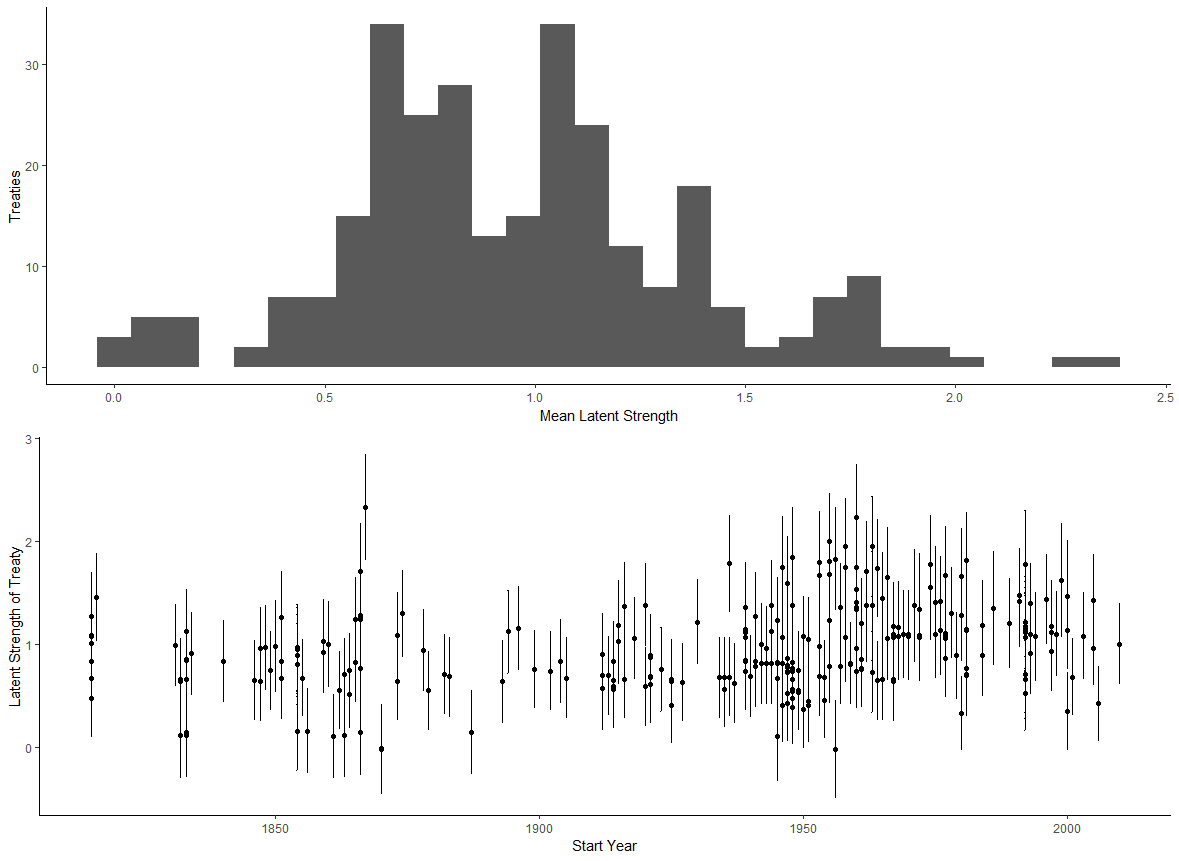
\includegraphics[width=0.95\textwidth]{../figures/ls-summary.png}
	\caption{Summary of latent measure of alliance treaty strength for 289 alliances promising military support from 1816 to 2016. The top panel is a histogram of the expected of alliance treaty strength. The bottom panel plots mean treaty strength (points) and the standard deviation (error bars) against the start year of the treaty.}
	\label{fig:ls-summary}
\end{figure}


% Cases- especially strong and weak treaties
The values of the latent strength measure are not intrinsically informative. 
Differences between treaties on the latent strength scale are meaningful, however. 
The mean of treaty strength is 0.92, and the median is 0.90. 
The median treaty is an 1854 agreement between Austria, France, and Britain against Russia in the Crimean war (ATOP ID 1180). 


The weakest treaty is an 1870 neutrality and offense pact between France and Britain (ATOPID 1300), which Britain used to protect Belgian neutrality during the Franco-Prussian war.  
Britain formed an identical with Prussia at the same time, which scores almost exactly the same on the latent measure. 
Both treaties have only offensive and neutrality promises, conditional on France and Prussia respecting Belgian neutrality. 


NATO (ATOPID 3180) has mean latent strength of 0.73, placing it in the second quartile of treaty strength. 
NATO's main costly provisions are the defense obligations in Article 5 and establishing a Council of members. 
According to the ATOP coding sheet for NATO, ``There are numerous bilateral agreements among NATO members re: military aid, bases, etc. but they do not qualify as separate alliances, nor are they part of the overall NATO structure.''
So while the NATO treaty is below average in strength, additional costs fall outside the formal treaty.    


The three strongest treaties are an 1867 alliance between Prussia and Hesse (ATOPID 1290), a 1955 treaty between Greece, Turkey and Cyprus (ATOPID 3400) and the United Arab Republic (ATOPID 3300).  
All these treaties supplement promises of military support with costly promises of cooperation. 
In the alliance between Greece, Turkey, and Cyprus, Greece and Turkey set up military aid, integrated military command, international organizations to mange relations on the island--- a weaker commitment would have lacked any credibility. 
These extra costs made commitments to defend Cyprus more credible. 


These examples show some face, concept, and discriminant validity of the latent measure. 
The UAR is a more costly commitment than a functional promise to respect Belgian neutrality. 
The weakest treaties make few costly promises beyond military support, matching my conceptualization of treaty strength. 
This measure makes a clear distinction between weak and strong commitments. 
I now describe how and why I use a multilevel model to estimate the association between this measure of treaty strength and alliance members' military spending.  


\subsection{Multilevel Model} 


% Best fit for theoretical process. Can compare alliances. 
Multilevel modeling incorporates elements of the specific and general research designs in previous research. 
Specific studies focus on responses to allied spending in particular treaties, while general studies in panel data rely on coarse aggregates of alliance participation.
In this model, I estimate the specific impact of each alliance on members' military spending as well as the general association between treaty strength and military expenditures. 
To facilitate computation and interpretation, I fit the multilevel model using Bayesian estimation in STAN \citep{Carpenteretal2016}.\footnote{See the appendix for details of the weakly informative prior distributions and evidence of convergence.}


The multilevel model is more complex than traditional approaches. 
But added complexity matches both the argument and data structure, while also generating novel inferences. 
Multilevel modeling connects the argument and research design. 
My predictions compare strong and weak treaties, so an alliance level regression in this multilevel model contains the corresponding coefficient.
Relying on a state-level proxy for alliance strength generates different comparisons and changes variation in the key independent variable.
Such aggregation may produce misleading inferences \citep{McElreath2016}. 


Multilevel modeling also matches the structure of the data.
Alliances and states are separate levels of analysis. 
Connecting the alliance and state level of analysis allows us to infer how alliance variation impacts states' military expenditures. 


Last, added complexity facilitates comparisons between alliances. 
An alliance-level regression estimates how multiple alliance characteristics are correlated with alliance strength and military spending.
Partial pooling produces reasonable estimates of the impact of each alliance on members' military spending. 
Comparing patterns in these alliance-specific coefficients provides additional evidence to examine Hypotheses 1 and 2 as well as the importance of treaty strength. 


\subsubsection{Model Summary} 

% Two separate but connected regressions
% State-level regression- alliances enter through spending matrix.
This multilevel model connects two distinct regressions. 
The base is a state-level regression, which is similar to a random effects panel data regression.
A second alliance-level regression predicts parameters in the state-level regression, like an interaction. 


The state-level regression starts with a distribution for the outcome:
\begin{equation}
y \sim student_t(\mu, \nu, \sigma)
\end{equation}
 
$y$ is growth in military spending. 
I model growth in spending using a t-distribution with degrees of freedom $\nu$ to address outliers.
$\sigma$ is analogous to the error term in a frequentist regression--- this captures unexplained variation in spending growth.  
$\mu$, the mean of the outcome, depends on several covariates.
\begin{equation}
\mu = \alpha + \alpha^{st} + \alpha^{yr} +\textbf{W} \gamma + \textbf{Z} \lambda
\end{equation}


Growth in spending is a function of an overall intercept $\alpha$, state and year varying intercepts $\alpha^{st}$ and $\alpha^{yr}$ and a matrix of state-level control variables $\textbf{W}$.
These components are a standard random effects model. 
The $\textbf{Z} \lambda$ term incorporates alliance participation.


$\textbf{Z}$ is a matrix of state participation in alliances. 
Columns correspond to alliances, and rows to state-year observations. 
If a state is not part of an alliance, the corresponding cell of the matrix is zero.
If a state is part of an alliance in a given year, the matrix cell contains the log of total allied military spending. 


I use total allied spending in the alliance participation matrix because more capable alliances provide extra benefits.
Increasing allied capability makes promises of military support more valuable \citep{Johnsonetal2015}.  
Treaty design then modifies the impact of allied capability.   
This measure also compares states inside and outside the treaty--- allied spending only applies to treaty members. 
So estimates of $\lambda$ also incorporate a change from no allied capability to some. 

Because the non-zero elements of $Z$ are allied spending, the $\lambda$ parameters capture alliance members' responsiveness to greater allied capability. 
Each alliance has a unique $\lambda$, which I give a common distribution. 
The shared distribution assumes alliances are similar but different in how they impact growth in military spending. 


% Alliance-level regression:
The second part of the multilevel model uses alliance characteristics to predict how allied spending is associated with growth in military spending. 
The $\lambda$ parameters are the dependent variable in an alliance-level regression which includes treaty strength.
Therefore, I focus interpretation on this alliance-level regression, where: 

\begin{equation}
\lambda \sim N(\theta, \sigma_{all})
\end{equation} 
and 
\begin{equation}
\theta = \alpha_{all} + \beta_1 \mbox{Treaty Strength} + \textbf{X} \beta
\end{equation}

% Like an interaction between alliance and state-level factors 
In this alliance-level regression, $\textbf{X}$ is a matrix of alliance-level control variables and $\alpha_{all}$ is the constant.
Adding $\sigma_{all}$ means predictions of $\lambda$ are not deterministic--- the alliance level regression contains an error term. 
Coefficients in the alliance-level regression are like marginal effects in an interaction. 
A change in treaty strength modifies $\lambda$, which alters growth in military spending.
Hypothesis 1 predicts $\beta_1$ will be negative among major powers, and Hypothesis 2 expects $\beta_1$ will be positive for non-major powers.  


% Provide an example observation
Consider one observation as an example of how the model works. 
Growth in Argentina's military spending in 1955 depends on Argentina's economic growth, political regime, conflict participation, and rival military spending. 
Argentine participation in the Rio Pact and OAS also changes growth in spending through allied capability. 


\begin{equation}
\begin{split}
& \mbox{Argentina 1955} = \mbox{Overall mean}
+ \mbox{Argentine Intercept} + \mbox{1955 Intercept} 
+ \mbox{Argentine Characteristics} \\
& + \lambda_{OAS} * \mbox{OAS Expenditure} + \lambda_{Rio} * \mbox{Rio Pact Expenditure}
\end{split} 
\end{equation}


$\lambda_{OAS}$ and $\lambda_{Rio}$ are modified by the alliance level regression. 
The institutional design and membership of these treaties alter the $\lambda$ parameter.
Alliances Argentina did not participate in have no impact on growth in military spending. 


The multilevel model is interactive, which is appropriate for my conditional argument. 
Alliance characteristics modify the impact of allied spending on growth in state military spending. 
I now describe the sample and covariates in the analysis.  



\subsection{Sample and Covariates} 

% Sample of states and alliances: latter is restricted to treaties with military support 
I estimate this model on two samples of states from 1816 to 2007--- one sample of major powers, the other of non-major powers. 
Alliance participation data comes from the ATOP project \citep{Leedsetal2002}. 
I focus on participation in defensive and offensive treaties, because prior studies of alliances and military spending examine these treaties. 


% Because I think the DGP is different for large and small- split sample.
My argument suggests that major and non-major powers use alliances for different purposes.
Major powers focus on influence, while non-major powers emphasize immediate territorial security.  
Therefore, the entire data-generating process connecting alliance participation and military spending is different for major and non-major powers. 
To capture these differences, I estimate the model in separate samples- one sample of major powers, the other of non-major powers.
I employ the classification of major power status from the Correlates of War Project. 


The non-major power sample contains 8,668 observations in the state-level regression, and 192 alliances. 
There are 930 major power observations and 148 alliances. 
Though the major power sample is smaller and has fewer states, Bayesian estimation and partial pooling should generate plausible estimates \citep{Stegmueller2013}. 

% DV: growth in milex
The dependent variable is growth in military spending.
I calculated growth in spending using the Correlates of War Project's measure of military spending \citep{SingerCINC1988}. 
Growth in spending is equal to changes in spending as a share of the previous year's military spending, so changes are relative to previous levels of spending. 


% Describe covariates at each level. 
In the state-level regression, I adjust for several variables that are correlated with of alliance participation and military spending. 
State-level covariates include GDP growth \citep{Boltetal2018}, regime type, international war \citep{Reiteretal2016}, civil war participation \citep{SarkeesWayman2010}, annual MIDs \citep{Gibleretal2016}, rival military spending \citep{ThompsonDreyer2012} and a dummy for Cold War years.
I include growth in GDP instead of levels of GDP because GDP levels are non-stationary, and economic growth shapes the opportunity costs of military spending \citep{Kimball2010, Zielinskietal2017}.


The alliance-level regression contains the mean of the latent treaty strength--- the key independent variable. 
Other alliance level variables include the number of members and share of democracies in a treaty at time of formation \citep{Chibaetal2015}.
I also control for superpower membership--- whether the US or USSR participated in a treaty during the Cold War. 
Two dummy indicators of wartime alliances and asymmetric obligations \citep{Leedsetal2002} complete the alliance-level regression specification. 
All these covariates are correlated with treaty strength and military spending. 


One control theoretically interesting as well. 
Democratic membership is a key theoretical quantity of interest, as prior studies find it is associated with limited obligations \citep{Chibaetal2015} and lower military spending \citep{DigiuseppePoast2016}.
This research design can establish whether democratic alliance membership reduces military spending after adjusting for alliance treaty strength. 
The next section describes the results.
 

\section{Results}


Results are based on 2,000 total samples from four chains, with 1,000 warm-up iterations. 
To facilitate model fitting, I employed a non-centered parameterization of the varying intercepts and a sparse matrix representation of \textbf{Z}. 
Standard convergence diagnostics indicate the chains adequately explored the posterior density.\footnote{See the appendix for more details on convergence.} 


% note on interpreting Bayesian results
Because I use Bayesian modeling to estimate the association between treaty strength and growth in military spending each coefficient has a posterior distribution--- the likely values of the coefficient conditional on the priors and observed data.
There are no conventional indicators of statistical significance. 
Instead I calculate the negative and positive posterior probability for the two treaty strength coefficients to assess Hypotheses 1 and 2.


% show latent strength coefficient in each subset of data
\begin{figure}[htbp]
	\centering
		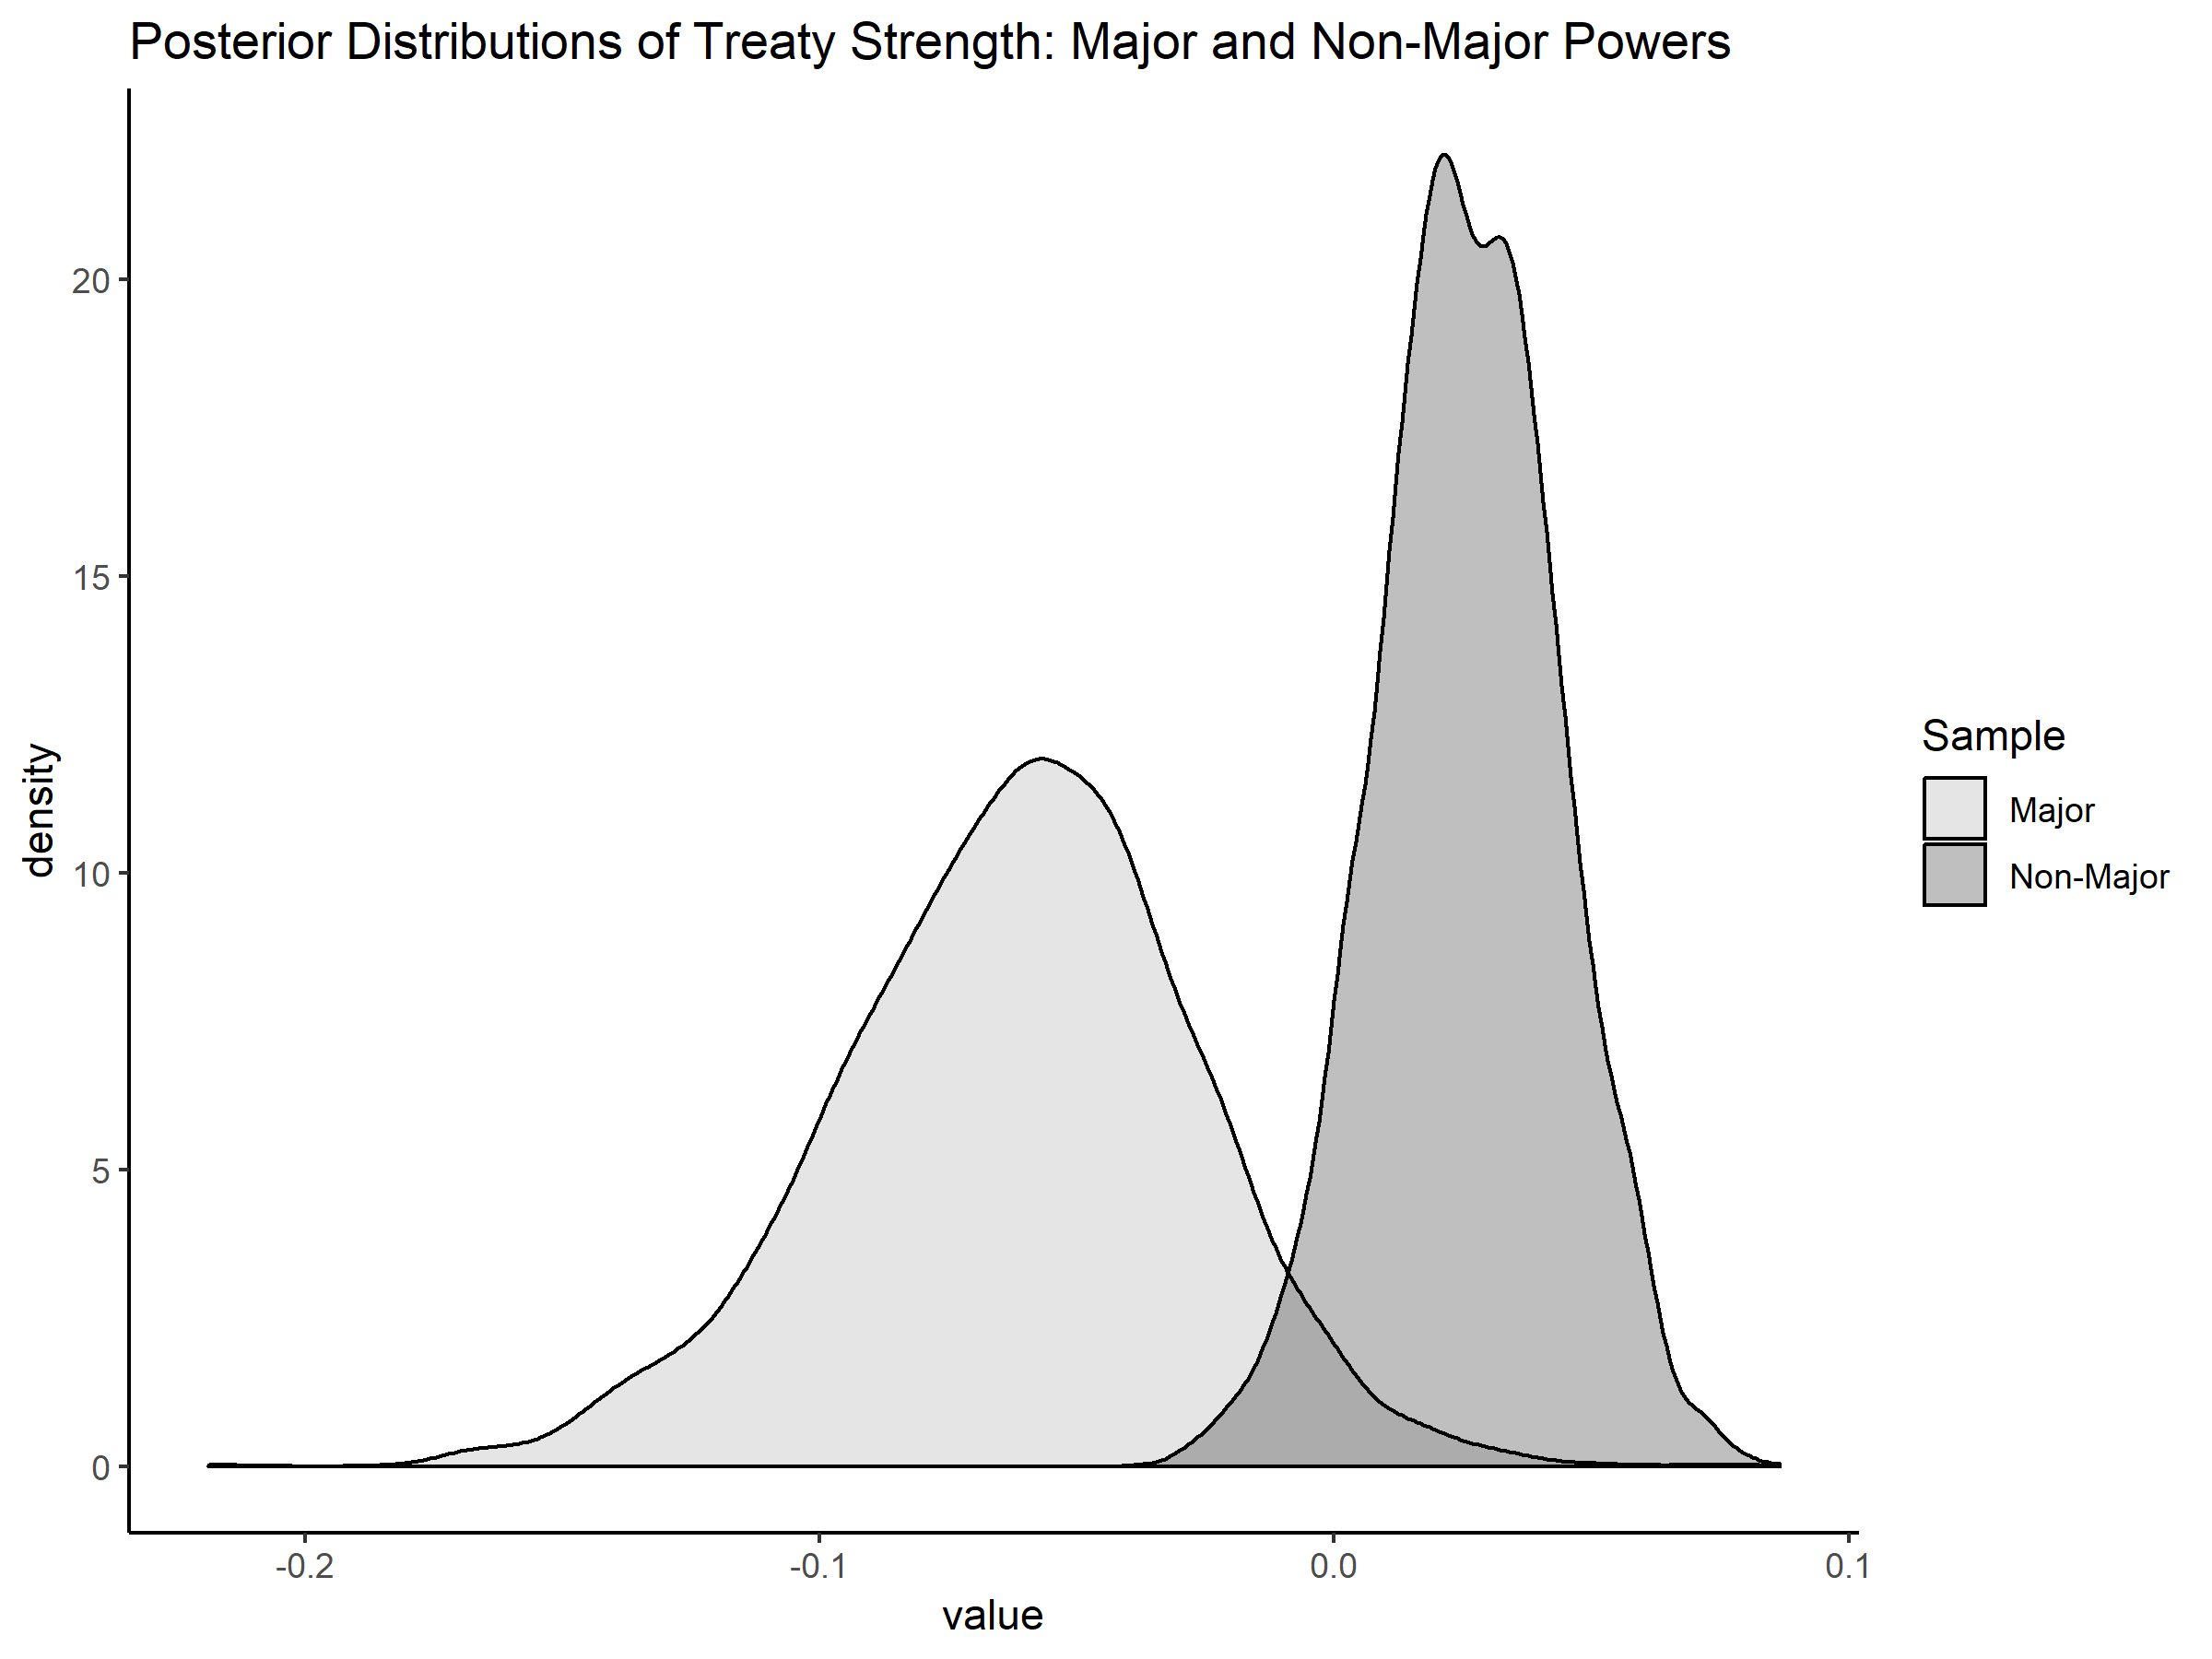
\includegraphics[width=0.95\textwidth]{../figures/str-dens.png}
	\caption{Posterior density of treaty strength coefficient in major and non-major power samples, 1816 to 2007. 96\% of the major power posterior mass is negative. 94\% of the non-major power posterior mass is positive.}
	\label{fig:str-dens}
\end{figure}


\autoref{fig:str-dens} plots the full posterior density of the treaty strength coefficients in the major and minor power samples.
\footnote{The smaller sample for major powers produces more variance in all the coefficient estimates.} 
96\% of the posterior mass for major powers is negative. 
94\% of the posterior mass for minor powers is positive. 
There is only 6\% overlap between these two posteriors. 


These two coefficient estimates match the predictions of Hypotheses 1 and 2. 
For major powers, there is a 96\% chance increasing treaty strength is associated with lower growth in military spending. 
There is a 94\% chance greater treaty strength is associated with higher growth in military spending for non-major powers.


How substantively important is treaty strength? 
Among major powers, the mean of the treaty strength coefficient is -0.05, and median growth in military expenditures is 0.04.
\footnote{The median is a better summary of the dependent variable because large positive and negative outliers influence the mean.} 
So a one-unit increase in treaty strength more than offsets the typical annual growth in military spending. 
This change in spending is a plausible effect--- 5.1\% of the 2018 US defense budget was spent directly on NATO.
\footnote{See this \href{https://www.iiss.org/blogs/military-balance/2018/07/us-and-nato-allies-costs-and-value}{blog post from the IISS}.} 


For non-major powers, the mean of the treaty strength coefficient is 0.03, and median growth in military expenditures is 0.06. 
Greater treaty strength increases growth in minor power military expenditures by about half of typical growth. 
In both the major and non-major power samples, higher treaty strength has a large substantive effect. 


We can also examine how much changing treaty strength influences on the overall association between changes in allied spending and growth in defense spending. 
Each $\lambda$ parameter measures the aggregate impact of changes in allied capability for a treaty. 
If greater treaty strength has a large influence on the $\lambda$ parameters, there will be a clear trend in the mean of $\lambda$ across the range of alliance treaty strength.
We should observe a negative trend in the expected value of $\lambda$ as treaty strength increases in major power alliances. 
There will be a positive trend in $\lambda$ for non-major power alliances. 


\begin{figure}[htbp]
	\centering
		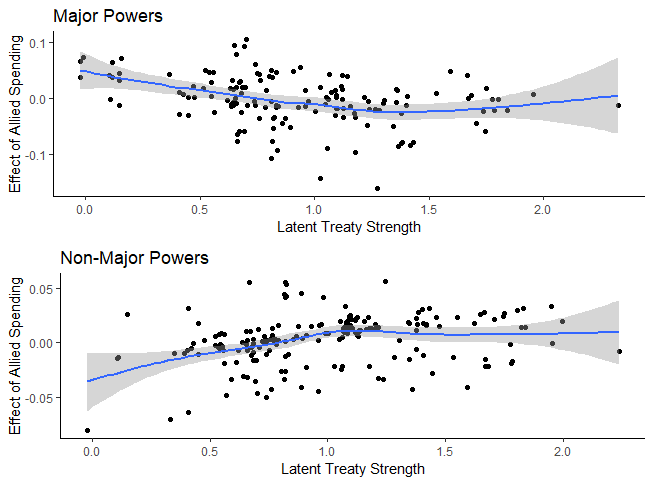
\includegraphics[width=0.95\textwidth]{../figures/lambda-ls-scatter.png}
	\caption{Scatter plots of trends in mean $\lambda$ parameters and treaty strength. $\lambda$ is the total impact of alliance participation on growth in military spending. The top panel is major powers, where this is a negative trend between $\lambda$ and treaty strength. In the bottom panel the same trend is positive for non-major powers. Trend lines estimated using linear regression.}
	\label{fig:lambda-ls-scatter}
\end{figure}


\autoref{fig:lambda-ls-scatter} plots the expected value of $\lambda$ against treaty strength in the two samples. 
In the major power sample, there is a negative trend in the scatter plot.
For non-major powers, the trend is positive.
The correlations between mean $\lambda$ and treaty strength are statistically significant in both samples. 


These trends match the underlying logic of Hypotheses 1 and 2. 
Weaker treaties tend to increase growth in defense spending for major powers, but that positive correlation falls as treaty strength increases. 
In non-major powers, the trend starts negative and becomes more positive as treaty strength rises. 
Because other treaty characteristics and unmeasured error also influence the $\lambda$ estimates, not all treaties conform to the expectations of decreasing or increasing growth in spending. 


Because $\lambda$ captures the total impact of an alliance, this pattern suggests that increasing treaty strength has an important role. 
Even after accounting for other alliance characteristics, alliance strength drives the overall effect of allied spending down for major powers, and up for non-major powers. 


While the statistical model provides novel empirical evidence, it does not show the underlying theoretical mechanisms. 
To illustrate the theoretical process, I offer brief case study evidence from US alliance politics in the next section.  
I focus on the case of NATO--- perhaps the most important alliance. 


\section{NATO, Treaty Strength and Military Spending}


US foreign policy after World War II also illustrates the tradeoff between entanglement and influence for major powers as well as the consequences of treaty design for junior partners. 
The US balanced between fear of ``foreign entanglements'' and maintaining influence. 
The extensive network of alliance commitments to contain the USSR required massive defense outlays \citep{Fordham1998}. 
These expenditures grew more due to weak formal alliance commitments.. 


% Look at strong US commitment to Iran
Most US treaties contain few formal promises besides defense against aggression. 
Fear of entanglement abroad led the US to form weaker treaties.
In turn, these limited formal promises required additional defense outlays.  
NATO is an excellent example of these dynamics. 


After the end of World War II, the US sought a way to protect Europe from the USSR. 
Isolationists in the US Senate feared that an alliance would force America to intervene automatically if partners were attacked, bypassing the power of Congress to declare war \citep[pg. 280-1]{Acheson1969}.
Therefore Article V states that if one member is attacked the others ``will assist the Party or Parties so attacked by taking forthwith, individually and in concert with the other Parties, \emph{such action as it deems necessary} (emphasis mine).'' 
Military support was and is not guaranteed. 


The absence of automatic US involvement increased demand for reassurance by European allies. 
Europeans feared that if the Soviets invaded, the US would decide not to fight. 
Therefore, bilateral agreements on troop deployments became an instrument of reassurance. 


In 1950 the Germans formally requested clarification on whether an attack on US forces in Germany would be treated as an armed attack on the US- which the US said it would \citep[pg. 395]{Acheson1969}. 
A 1951 presentation by Dean Acheson to Dwight Eisenhower argued European allies ``fear the inconstancy of United States purpose in Europe. ... These European fears and apprehensions can only be overcome if we make the necessary full and active contribution in terms of both military forces and economic aid'' \citep[pg. 3]{Acheson1951}.  
Even after agreeing to deploy troops, US policymakers hoped Europeans would soon provide more for their own defense, while acknowledging the US ``should not dictate what they shall do'' \citep[pg. 2]{Johnson1950}. 


The US also included few sunk costs promises in the NATO treaty. 
Many Senators also opposed military aid to Europe \citep[pg 285]{Acheson1969}, leading to more bilateral bargaining and aid through other channels. 
As a result, the US has less formal leverage in NATO than is commonly thought. 


American policymakers frequently attempt to browbeat NATO members into spending more. 
These shaming efforts have usually failed. 
Most European members of NATO have been unresponsive to changes in external threat and US defense spending \citep{PluemperNeumayer2015}. 


The US has threatened to leave NATO in response to European ``free-riding,'' but those threats were not credible. 
During the Cold War, US interests in containing the USSR trumped irritation with allied free-riding.  
But without other formal treaty commitments to influence NATO members, the US had few ways besides public statements to check allied desires to reduce growth in military spending. 


% add something on estimates from ML model
Estimates of the $\lambda$ parameter in the major and non-major power samples match this reading of the NATO case. 
In the major power sample, NATO membership adds 0.04 to growth in military spending in expectation.
For non-major powers, NATO membership lowers growth in military expenditure by -0.006 in expectation.\footnote{
The UK and France are major powers from 1945 on, and Germany is coded as a major power by the Correlates of War after 1991. Therefore, these estimates may underestimate lower growth in spending by NATO members, because all three of these states relied on US capability for protection. The positive growth in major power spending is almost certainly driven by the US. In a future iteration of this paper, I will expand the typology of capability to include superpowers.
}
So the statistical analysis predicts greater growth for major powers and reduced growth for non-major powers from NATO membership.  


% Sum up 
NATO is the most important alliance in international relations. 
US fear of entanglement led to a need for growth in military spending and limited bargaining leverage in alliance maintenance. 
European members still gained security, but retained the freedom of action to lower growth in defense spending. 
This case matches the results of the multilevel model, illustrating the heterogeneous effects of treaty strength on major and non-major powers. 


\section{Discussion}


% Matches argument 
The results of the statistical analysis conform to expectations of Hypotheses 1 and 2. 
Increasing treaty strength is positively associated with growth in military spending in non-major powers. 
Greater treaty strength is associated with lower growth in military spending for major powers, who use treaty strength and military capability as substitutes while seeking influence. 


% Precise interpretation: compares strong and weak alliances. Not treaty vs absence. 
These results contribute to the debate over whether alliance participation increases or decreases military spending. 
Dissension between the force multiplier and foreign entanglement views of alliances is based on competing claims about the purposes of alliances. 
This dispute omits crucial differences between states and alliances. 


My findings and argument suggest claims alliance participation only increases or decreases military spending are inappropriate. 
The association between alliance participation and growth in military spending depends on alliance member size and treaty strength. 
Alliance participation has heterogeneous effects because major powers and non-major powers employ treaties for different purposes. 


% Link for force multiplier and foreign entanglement
The force multiplier perspective applies best to non-major powers. 
But these states cannot reduce growth in military spending in all alliances, because strong treaties constrain their freedom of action.
Alliances are a foreign entanglement for major powers. 
But additional entanglement in a strong treaty provides more influence, attenuating the positive correlation between alliance participation and growth in military spending. 


How do my results compare to other evidence on alliance participation and military spending? 
Connecting my findings with prior evidence requires renewed attention to specific and general research designs. 
General studies compare states in a particular kind of alliances to those outside the treaty. 
Specific studies estimate responsiveness to allied military spending. 


My research design incorporates both treaty presence and changes in allied capability through the matrix of alliance participation. 
$\lambda$ measures the impact of increasing allied spending \textit{for states in a treaty}. 
Thus, $\lambda$ includes shifts from no to some allied capability as well as changes in allied capability while states are members.
Alliance participation is both treaty presence (formation) and changes in allied capability (maintenance). 


The key coefficient estimates compare strong and weak treaties in the alliance-level regression. 
The alliance-level coefficient estimates are like marginal effects- increasing treaty strength alters the effect of alliance participation.
Greater treaty strength decreases the association between alliance participation and growth in military expenditures for major powers, and increases it for non-major powers. 
Therefore, my results encompass specific and general studies in a unified framework. 


% limitations of RD
This paper has several limitations.
The argument does not address the domestic political economy of military spending. 
My argument reduces domestic politics to an assumption that military spending has opportunity costs, which are decreasing in state size. 


In the research design, the COW measures of military spending contain substantial measurement error. 
There is also a great deal of missing data in the 1816--2007 time frame of this study. 
I plan to check the robustness of my results to these issues by adding measurement error to the outcome and imputing missing data.


The multilevel model only incorporates time-invariant alliance characteristics, save for changing capabilities in the membership matrix. 
So I measure share of democratic members and the number of members at time of formation. 
Allowing time-varying alliance characteristics might improve the statistical model, but would require altering the model structure. 


% Strategic treaty design
Strategic alliance design is the last major weakness of the research design. 
Non-random selection into different kinds of alliances might produce systematic differences between members that are no adjusted for in my statistical model. 
I attempted to control for correlates of alliance treaty strength, especially democracy, but oversights are possible. 



\section{Conclusion}


% Start conclusion 
This paper presented an argument and empirical evidence linking alliance participation and military expenditures. 
I explain when alliance participation is associated more or less growth in military spending, addressing a debate between the force multiplier and foreign entanglement views of alliances. 
Whether alliance participation increases or decreases military spending depends on state capability and alliance treaty strength. 
For major powers, greater treaty strength leads to lower growth in spending. 
Non-major power growth in spending is positively correlated with alliance treaty strength. 
I provide evidence for these predictions using a new measure of alliance treaty strength and a multilevel model. 


% Add paragraph on distributional consequences.
Changes in military spending from alliance participation have important distributional consequences. 
By altering growth in military spending, the design of international alliances alters the domestic political economy of member states. 
Non-major powers confront the opportunity costs of additional defense spending in strong treaties.
Major powers can use strong treaties to reduce to domestic costs of their foreign policy ambitions.  


% Next steps: extend argument to other treaty characteristics
There are several next steps for research on alliances and military expenditures. 
One is extending the argument to other alliance characteristics. 
If major and non-major powers employ alliances for different ends, then other alliance characteristics may have different impacts on military spending. 
Large and small states should use wartime and asymmetric treaties differently, for instance. 


% Next steps: More interp of lambdas
Another task for future research is making more detailed comparisons of the $\lambda$ parameters. 
Each $\lambda$ captures the aggregate impact of alliance participation for individual treaties.
As such, these parameters are a novel measurement, and additional evidence of when alliance participation increases or decreases military spending. 


% Case studies
The multilevel regression estimates alone do not establish causality \citep{Seawright2016}. 
But the $\lambda$ parameters can guide case selection in process-tracing to corroborate the regression results.
One possible design is selecting the five largest and smallest $\lambda$ values for major and minor powers, and determining whether the connection between alliance participation and military expenditures matches the theoretical process.


% ML model and other cases of multiple membership 
The research design in this paper applies to other international relations questions.
If scholars are interested in a class of international organizations and states are members in multiple organizations, the multilevel model incorporates multiple membership.
For example, international political economy scholars could apply this model to trade agreements. 
Studies of international law could examine the impact of membership in different conventions and international organizations on human rights. 


% The argument indicates tradeoff
The argument and evidence suggests that major and non-major powers each face a tradeoff in alliance treaty design. 
Major powers tradeoff between entanglement and greater influence in strong treaties. 
Non-major powers sacrifice freedom of action for greater security as treaty strength rises. 


% Implications for policy. 
These twin tradeoffs have important consequences for policy debates.
The United States has often decried ``free-riding'' by allies who provide too little for their own defense \citep{Lanoszka2015}. 
But allies are able to free-ride because the US makes relatively weak formal alliance commitments. 
``Entangling alliances'' may provide more influence to curb falling allied defense spending. 

 
Therefore, growing institutionalization of NATO, including the agreement for all allies to spend at least 2\% of GDP on defense, may be effective. 
However, treating alliances between major and non-major powers as a public good and treating low defense effort as free riding, is inappropriate. 
Asymmetric alliances produce different goods for different members. 
Major powers seek influence, while non-major powers secure their homeland. 


The US could use stronger formal commitments as a substitute for greater defense effort in reassuring allies.
The danger is that making stronger commitments could create a situation where obligations exceed capabilities \citep{Kennedy1987}. 
Emboldening junior partners with a strong treaty might have deterrent value \citep{Bensonetal2014}, or increase the risk of conflict \citep{Benson2012}. 

 
% tie it all together
The connection between alliance participation and military expenditures depends on state size and the strength of the treaty.  
Alliance participation does not exclusively increase or decrease military spending.  
Both the force multiplier and foreign entanglement views of alliance participation are correct, each in different circumstances. 




\singlespace
 
\bibliography{../../MasterBibliography} 





\end{document}
